\documentclass[russian]{article}
\usepackage[T1]{fontenc}
\usepackage[utf8]{inputenc}
\usepackage{geometry}
\geometry{verbose,tmargin=2cm,bmargin=2cm,lmargin=1cm,rmargin=1cm}
\usepackage{float}
\usepackage{textcomp}
\usepackage{amssymb}
\usepackage{graphicx}
\usepackage{babel}
\usepackage[T2A]{fontenc}

\makeatletter
\@ifundefined{date}{}{\date{}}


\begin{document}

\title{Матлогика. HW\#5}
\author{Тураев Тимур, 504 (SE)}

\maketitle

\paragraph{1} \textit{Доказать, что существует $k\in \mathbb{N}$, такое что неразрешимо множество \[ H^k = \{ x | \langle k \rangle (x) \neq \bot \} \]}

На самом деле не очень понятно как решать. Примеры из лекции и из практики мне ясны, а вот как приложить их к этому примеру, я не знаю…

\paragraph{2} \textit{Сигнатура $(f^1, =^2)$, носитель $\mathbb{Z}$, нормальная интерпретация, $[f](x) = x + 2$. Невыразимый предикат $y = x + 1$. Найдите автоморфизм, относительно которого данный предикат неустойчив.}

Предлагается такой автоморфизм: $x \rightarrow x \bmod 2$. То есть автоморфизм, сохраняющий четность. Это действительно автоморфизм (проверить легко).
Предикат $y = x + 1$, ясно, неустойчив: $+1$ в правой части меняет четность.

\paragraph{3} \textit{Сигнатура $(=^2, P^2)$, носитель $\mathbb{N}_+$, нормальная интерпретация, $[P](x, y) = x | y$. Невыразимый предикат $x = 2$. Найдите автоморфизм, относительно которого данный предикат неустойчив.}

Предлагается такой автоморфизм: $x \rightarrow 2x$. Это действительно автоморфизм (проверить легко).
Предикат $x = 2$, ясно, неустойчив: из того, что $x=2$ не следует что $2x = 2$ внутри носителя $\mathbb{N}_+$

\paragraph{4} \textit{Построить дерево вывода.
\[
\vdash \exists y \forall x Q(x,y) \rightarrow \exists x Q(x, x)
\]}

\begin{center}
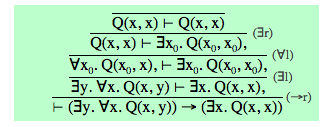
\includegraphics[scale=0.64]{4.png} 
\end{center}

\paragraph{5} \textit{Построить дерево вывода.
\[
\vdash \exists x (P(y) \vee P(f(z)) \rightarrow P(x))
\]}

\begin{center}
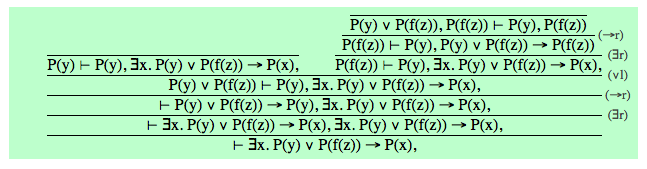
\includegraphics[scale=0.64]{5.png} 
\end{center}

\paragraph{6} \textit{Построить дерево вывода.
\[
\vdash \exists x \forall y (P(x) \rightarrow P(y))
\]}

\begin{center}
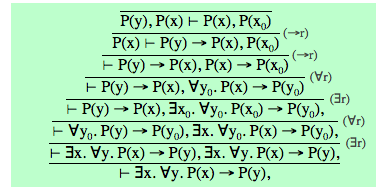
\includegraphics[scale=0.64]{6.png} 
\end{center}

\end{document}
